\section{Теоретическая часть}

\textbf{Переходные процессы} — процессы, возникающие в электрических цепях при различных воздействиях, приводящих их из стационарного состояния в новое стационарное состояние, то есть, — при действии различного рода коммутационной аппаратуры, например, ключей, переключателей для включения или отключения источника или приёмника энергии, при обрывах в цепи, при коротких замыканиях отдельных участков цепи и т. д.

Например, при подключении разряженного конденсатора $С$ к источнику напряжения $U_0$ через резистор $R$ напряжение на конденсаторе меняется от 0 до $U_0$ по закону:

\[
U_C (t) = U_0(1-e^{-\frac{t}{\tau}}), \tau = R \cdot C
\]

Физическая причина возникновения переходных процессов в цепях — наличие в них индуктивных и ёмкостных элементов в соответствующих схемах замещения. Объясняется это тем, что энергия магнитного и электрического полей этих элементов не может изменяться скачком при коммутации в цепи. 

Фильтры высоких и низких частот — это электрические цепи, состоящие из элементов, обладающих нелинейной АЧХ — имеющих разное сопротивление на разных частотах.

Частота среза — частота, выше или ниже которой мощность выходного сигнала некоторого линейного частотно-зависимого объекта уменьшается в два раза от мощности в полосе пропускания при воздействии на вход неизменного по амплитуде сигнала. 

Амплитудно-частотная характеристика на частоте среза имеет спад до уровня -3дБ относительно уровня в полосе пропускания. 

Частотные фильтры изготавливаются из элементов, обладающих реактивными сопротивлениями – конденсаторов и катушек индуктивности. Реактивные сопротивления, используемых в фильтрах конденсаторов и катушек индуктивности связаны с частотой ниже приведёнными формулами:

\[
X_c = \frac{1}{\omega \cdot C} = \frac{1}{2 \pi f C}, X_L = \omega L = 2 \pi f L
\]

\begin{figure}[H]
	\centering
	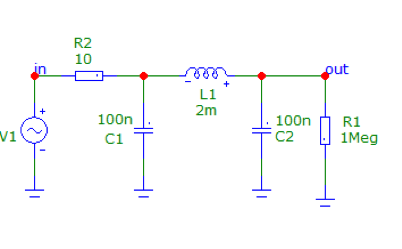
\includegraphics[width=0.7\linewidth]{img/f1}
	\caption{П-образный низкочастотный фильтр}
\end{figure}

\begin{figure}[H]
	\centering
	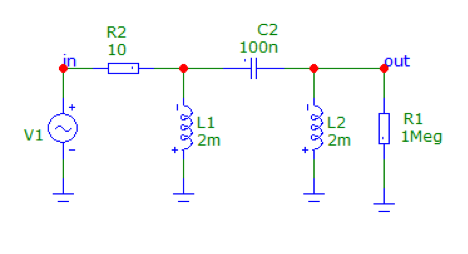
\includegraphics[width=0.7\linewidth]{img/f2}
	\caption{П-образный высокочастотный фильтр}
\end{figure}

\begin{figure}[H]
	\centering
	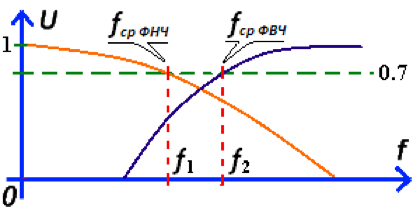
\includegraphics[width=0.7\linewidth]{img/f3}
	\caption{Частота среза ФНЧ и ФВЧ}
\end{figure}

\section{Модель в microcap}

Моделирование высокочастотного фильтра, выполненного в microcap, представлено на рисунке 4, АЧХ – на рисунке 5

\begin{figure}[H]
	\centering
	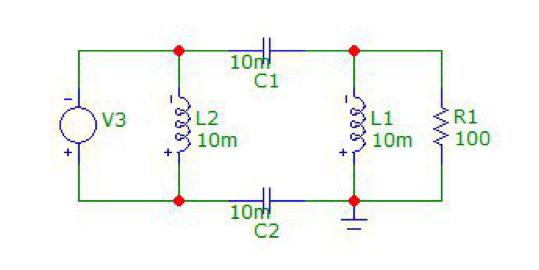
\includegraphics[width=0.7\linewidth]{img/f4}
	\caption{ФВЧ}
\end{figure}

\begin{figure}[H]
	\centering
	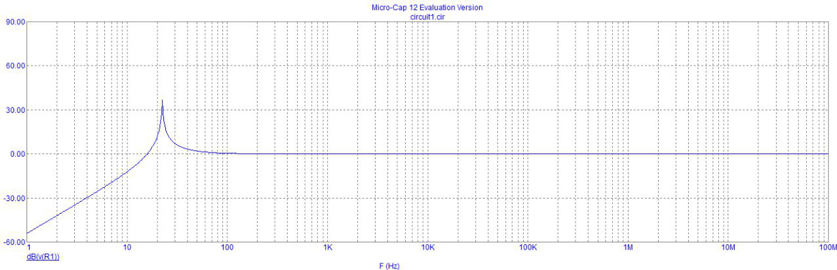
\includegraphics[width=0.7\linewidth]{img/f5}
	\caption{АЧХ ФВЧ}
\end{figure}

Моделирование низкочастотного фильтра, выполненного в microcap, представлено на рисунке 6, АЧХ – на рисунке 7.  

\begin{figure}[H]
	\centering
	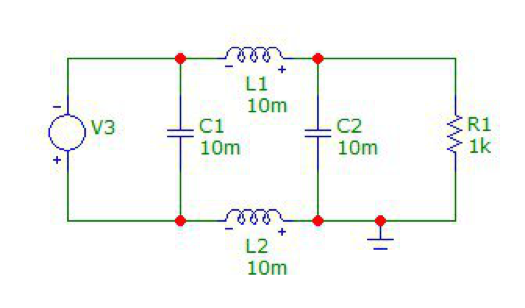
\includegraphics[width=0.7\linewidth]{img/f6}
	\caption{ФНЧ}
\end{figure}

\begin{figure}[H]
	\centering
	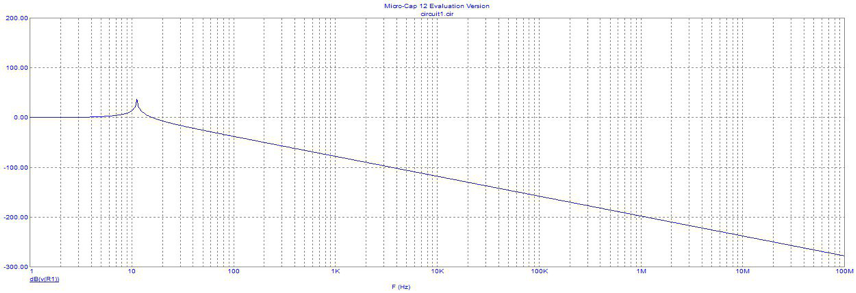
\includegraphics[width=0.7\linewidth]{img/f7}
	\caption{АЧХ ФНЧ}
\end{figure}

Моделирование схемы с генератором, выполненного в microcap, представлено на рисунке 8, выходные характеристики – на рисунке 9.  

\begin{figure}[H]
	\centering
	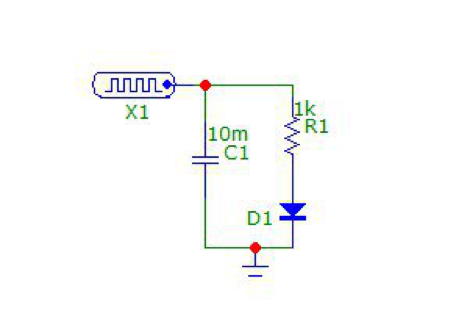
\includegraphics[width=0.7\linewidth]{img/f8}
	\caption{ФНЧ}
\end{figure}

\begin{figure}[H]
	\centering
	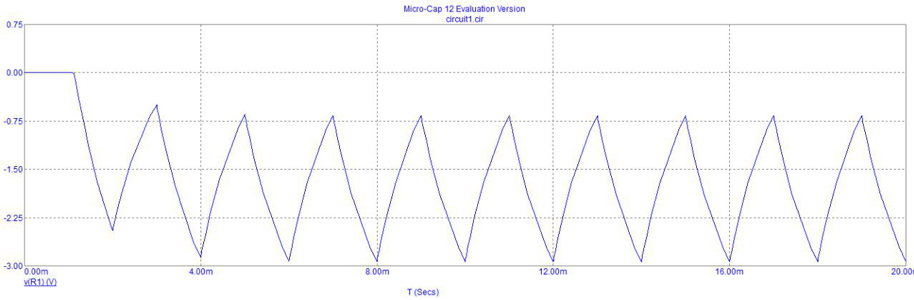
\includegraphics[width=0.7\linewidth]{img/f9}
	\caption{АЧХ ФНЧ}
\end{figure}

\section{Блок-схема измерительной установки}

\begin{figure}[H]
	\centering
	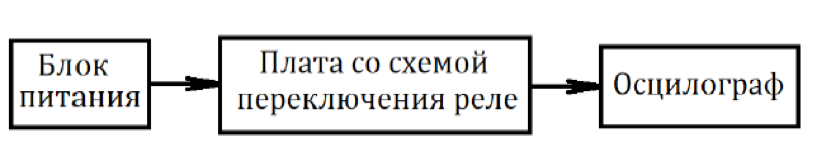
\includegraphics[width=0.7\linewidth]{img/f10}
	\caption{Блок-схема установки для исследования переходных процессов}
\end{figure}

\begin{figure}[H]
	\centering
	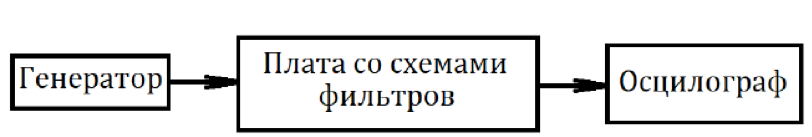
\includegraphics[width=0.7\linewidth]{img/f11}
	\caption{Блок-схема установки для исследования низкочастотного и высокочастотного фильтров}
\end{figure}

\section{Результаты измерения, полученные в ходе выполнения лабораторной работы}

Измерения напряжений $U_1$ и $U_2$ в двух различных моментах времени $t_1$ и $t_2$ представлены в таблице 1.

\begin{table}[H]
	\centering
	\begin{tabular}{|c|c|c|}
		\hline
		& t,  мс & U, В \\ \hline
		1 & 10     & 1.5  \\ \hline
		2 & 30     & 2.33 \\ \hline
	\end{tabular}
\end{table}

На рисунке 12 представлены результаты работы осциллографа.

\begin{figure}[H]
	\centering
	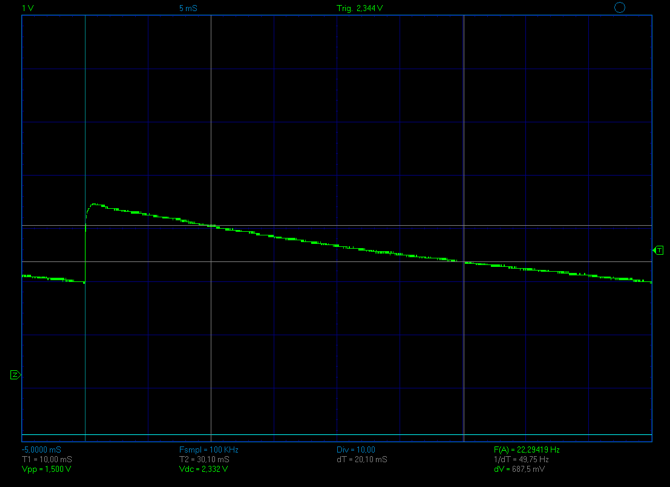
\includegraphics[width=0.7\linewidth]{img/f12}
	\caption{Результаты работы}
\end{figure}





